\chapter{Proposta}

% Obs: MM = Monitoramento de Memória

% ------------------------------------

% 1. (Prof. Paulo) Como será feita a coleta das métricas dos servidores?
% R. A coleta será feita por meio de requisições ao sistema operacional, diretamente.

% 2. (Prof. Paulo) Qual será a frequência da coleta?
% R. Foram definidos três períodos distintos de coleta e atualização dos dados - 6s, 60s (1 min) e 600s (10min), com o propósito de avaliar, em diferentes ordens de grandeza, o impacto da obsolescência de dados no monitoramento.

% 3. (Prof. Paulo) Como será o monitoramento - Que comando será utilizado? Será criado um programa que coleta o uso de memória?
% R. Nos servidores, haverá uma aplicação que periodicamente usa o sistema operacional para obter dados de consumo de memória (conforme as frequências de teste definidas anteriormente).

% 4. (Prof. Paulo) Como o balanceador de carga obterá as métricas?
% R. A própria aplicação de balanceamento de carga estará inscrita (subscriber) em um broker MQTT que periodicamente receberá eventos de atualização dos dados. Reagindo à esse evento, o balanceador de carga atualiza seus dados periodicamente.

% 5. (Prof. Paulo) Como as métricas serão utilizadas no critério de decisão do balanceador de carga (algoritmo)?
% R. A ser definido (memória x disco), interpretação de dados obsoletos;

% 6. (Prof. Paulo) Como serão os cenários de testes?
% R. Análise perceptiva do travamento de vídeos (QoE final) usando round-robin, seleção aleatória, MM 6s, MM 60s, MM 600s (todos com técnicas de interpretação de dados obsoletos).

% 7. (Prof. Paulo) Qual será a topologia dos testes?
% R. Apenas uma rede virtual containerizada com alguns servidores e uma aplicação balanceadora de carga. O balanceamento será feito à nível de aplicação.

% 8. (Prof. Paulo) Um balanceador de carga será instrumentado para alcançar os objetivos?
% R. Uma aplicação simples será implementada para esse propósito. 

% 9. (Prof. Paulo) A coleta da informação pelo balanceador de carga e a tomada de decisão irão atrasar em quanto tempo o encaminhamento dos pacotes? Esse atraso irá impactar na qualidade?
% R. A escolha do protocolo MQTT foi feita justamente para este propósito, por ser leve. Espera-se que o impacto maior seja nos período menor (6s), uma vez que demandará maior tempo de processamento do balanceador de carga.  

% 10. (Prof. Paulo) O monitoramento de memória irá aumentar o consumo de outros recursos além da própria memória principal e secundária?
% R. De maneira análoga, espera-se que apenas que o consumo de CPU seja aumentado e com mais intensidade no período menor (6s) visto que as chamadas às APIs do sistema operacional serão mais frequentes.

% Adicional: Colocar aqui, na metodologia (diluído em outras partes) o referencial teórico do artigo "Interpreting Stale Load Information" de modo a obter respostas referenciadas para as perguntas 9 e 10 e fundamentar o algoritmo utilizado (pergunta 5).

% ------------------------------------

Esta seção aborda pormenorizadamente os caminhos escolhidos para a implementação do modelo de balanceamento de carga, bem como os métodos que serão utilizados para realizar a avaliação dos resultados finais.

% (OE 6) Estabelecer, conceitualmente, algoritmo de escolha de servidores por parte do balanceador de carga com base nos dados históricos fornecidos
\section{O algoritmo}

O primeiro passo, crucial para a determinação do modelo de otimização de balanceadores de carga, é a definição do algoritmo de balanceamento. Basicamente, a tarefa principal de um algoritmo de balanceamento de carga é o modo como a escolha do servidor será feita em cada requisição que chega ao sistema balanceador de carga.

Em particular, o algoritmo escolhido será \textbf{probabilístico}. Isso significa que, para cada servidor que poderá ser escolhido no processo, haverá uma probabilidade intrínseca baseada em parâmetros tanto individuais quanto gerais, e a estratégia de determinação dessa probabilidade é o que definirá o algoritmo em si. De acordo com o objetivo principal do trabalho, as duas principais (mas não únicas) métricas que exercerão influência sobre a determinação da probabilidade de escolha de cada servidor são o \textbf{consumo de memória RAM} e a \textbf{Taxa de Entrada e Saída de Disco}. Essas duas métricas são essenciais e vitais dentro do contexto de servidores que distribuem conteúdo, uma vez que sua única tarefa é recuperar estes arquivos do disco e efetivamente entregá-los ao solicitante. 

Em paralelo, os servidores enviarão, periodicamente, os dados de monitoramento referentes ao consumo de memória principal e à taxa de leitura de disco. A ideia é que o balanceador mantenha uma estrutura dinâmica que será atualizada de forma contínua, atualizando os parâmetros necessários e efetivamente promovendo eficiência na distribuição das requisições. O método que será usado para realizar a implementação deste conceito, bem como a definição das taxas de atualização dos dados dos servidores para o balanceador de carga, serão discutidos posteriormente.

A Equação \mbox{\ref{eq:basic_li}} utilizada no algoritmo corresponde a uma versão adaptada do \textit{Basic LI} \cite{interpretingStaleLoadInformation2000} de modo que, dada uma requisição, a determinação da probabilidade de escolha de um servidor $P{i}$ será determinada de acordo com seus parâmetros, onde:

\begin{enumerate}
    %\item[$T$]: Tempo médio de obsolescência da informação de carga, em unidades de tempo de serviço por tarefa.
    \item[$n$]: Número do total de servidores.
    %\item[$\lambda$]: Taxa média de chegada de requisições por servidor, como uma fração da vazão máxima do servidor. 
    \item[$L_{i}$]: Carga reportada no servidor $i$ (cálculo determinado na Equação \ref{eq:limemory}). 
    \item[$L_{tot}$]: Soma de todas as cargas reportadas ($\sum L_i$). 
    \item[$arrive_T$]: Número esperado de requisições que chegarão para o balanceador de carga durante um período de tempo $T$, que corresponde ao \textit{lifetime} (tempo de vida) médio das informações de carga de cada servidor.
    \item[$P_i$]: Probabilidade de que uma requisição que chega seja enviada para o servidor $i$. 
\end{enumerate}

\begin{gather} \label{eq:basic_li}
P_{i}=\frac{\frac{L_{tot}+arrive_{T}}{n}-L_{i}}{arrive_{T}}
\end{gather}

Note-se que no contexto do trabalho \cite{interpretingStaleLoadInformation2000}, "carga" é um termo genérico e abstrato. Para fins de implementação e aderência com o problema proposto por este trabalho, o parâmetro de carga ($L_i$ e consequentemente $L_{tot}$), aplicado na Equação \mbox{\ref{eq:basic_li}}, será calculado previamente através da coleta periódica das métricas de consumo de memória RAM e taxa de entrada e saída de memória secundária (cujo processo será descrito posteriormente), da normalização desses parâmetros em pontos percentuais e, finalmente, da mesclagem desses parâmetros para que possam ser inseridos na fórmula. Nesse sentido, a carga de um servidor ($L_i$) será determinada considerando:

\begin{enumerate}
    \item[$n$]: Número do total de servidores.
    \item[$LM_i$]: Consumo de memória principal no servidor $i$, representando a quantidade de memória usada para transferir o conteúdo no tempo T, normalizado em pontos percentuais com relação à capacidade total de memória do servidor $i$.
    \item[$LD_i$]: Carga do disco no servidor $i$, representando a velocidade do fluxo de busca e leitura das informações do disco no tempo T, normalizada em pontos percentuais com relação a capacidade total de leitura do disco no servidor $i$.
    \item[$TM$]: Taxa de uso geral de memória, determinado por $\sum_{i=0}^n \frac{LM_i}{n}$.
    \item[$TD$]: Taxa de consumo geral de operações de disco, determinado por $\sum_{i=0}^n \frac{LD_i}{n}$. 
\end{enumerate}

Sendo assim, a Equação \mbox{\ref{eq:limemory}} define a carga, no contexto deste trabalho, de um servidor de conteúdo.

\begin{gather} \label{eq:limemory}
    L_i = CM * LM_i + CD * LD_i
\end{gather}

Nesse contexto, $CM$ e $CD$ são coeficientes que multiplicam as suas respectivas cargas normalizadas. Eles são definidos de acordo com as Equações \mbox{\ref{eq:cm}} e \mbox{\ref{eq:cd}}, respectivamente, e representam a fração normalizada de memória e disco totais, respectivamente, em relação ao total conjugado de memória e disco.

\begin{gather} \label{eq:cm}
    CM = \frac{TM}{TM + TD}
\end{gather}

\begin{gather} \label{eq:cd}
    CD = \frac{TD}{TM + TD}
\end{gather}

Os coeficientes $CM$ e $CD$ são valores entre $0$ e $1$ de modo que $CM + CD = 1$. Eles são determinados dessa forma para que o recurso computacional que mais esteja sendo utilizado de modo geral em todos os servidores efetivamente contribua mais para o valor da carga de cada servidor $L_i$, de forma diretamente proporcional à taxa de consumo de cada um dos parâmetros. Finalmente, para que o sistema efetivamente esteja apto para calcular o valor de cada servidor $L_i$, basta que ele obtenha os valores de $LM_i$ e $LD_i$ de todos os servidores. Com eles, será possível calcular primeiramente $TM$ e $TD$, e, com esses valores, calcular $CM$ e $CD$ dinamicamente.

O algoritmo é executado a cada nova requisição que chega ao balanceador. Ele utiliza os dados de carga pré-calculados para determinar dinamicamente a probabilidade ($P_i$) de cada servidor ser escolhido, aplicando a Equação 1. Com as probabilidades definidas, ele emprega um método de seleção aleatória ponderada para despachar a requisição, garantindo que servidores menos sobrecarregados tenham maior chance de serem selecionados. O seguinte pseudocódigo descreve seu funcionamento.


\begin{algorithm}[H]
\caption{Seleção de Servidor por Requisição}
\begin{algorithmic}[1]
\Statex \textbf{Gatilho}: Chegada de uma nova requisição $R$.
\Require
    \Statex $S$: Lista de servidores com métricas $L_i$ e $T_i$ atualizadas.
    \Statex Variáveis globais: $L_{tot}, n$.
\Ensure
    \Statex Requisição $R$ encaminhada para um servidor $S_{i}$.

\Procedure{SelecionarServidor}{$R, S, L_{tot}, n$}
    \State $T \leftarrow \text{CalcularMediaDeRequisicoes}(S)$
    \State $arrive_T \leftarrow \text{CalcularChegadasEsperadas}(T)$
    \State $P_{list} \leftarrow []$ \Comment{Lista de probabilidades}
    
    \ForAll{$S_i, L_i$ in $S$}
        \State $numerador \leftarrow (L_{tot} + arrive_T)/n - L_i$
        \State $P_i \leftarrow ((L_{tot} + arrive_T)/n - L_i) / arrive_T$ \Comment{Eq. \ref{eq:basic_li}}
        \State Adicionar $(S_i, P_i)$ a $P_{list}$
    \EndFor
    
    \State $s_{escolhido} \leftarrow \text{SelecaoAleatoriaComPesos}(P_{list})$
    \State \text{Encaminhar}(R, $s_{escolhido}$)
\EndProcedure
\end{algorithmic}
\end{algorithm}

% As duas variáveis globais necessárias para o funcionamento do algoritmo são $L_{tot}$ e $n$. Ambas são recalculadas durante a chegada de cada informação enviada de um dos servidores ao balanceador de carga e a detecção de novos servidores pode ser feita de forma automática por meio de um evento que caracteriza a entrada de um novo servidor no \textit{pool} de serviços através de uma identificação ainda não realizada. Dessa forma, é possível obter elasticidade, deterministicamente adicionando um novo serviço caso chegue um evento com sua identificação e heuristicamente removendo serviços usando um valor arbitrário de \textit{threshold} equivalente ao tempo sem receber atualizações daquele servidor.

Para o funcionamento do algoritmo, são empregadas duas variáveis globais: $L_{tot}$ e $n$. Ambas são variáveis dinâmicas e automaticamente recalculadas sempre que o balanceador de carga recebe informações de qualquer servidor. A detecção de novos servidores ocorre de forma automática e determinística quando um evento caracteriza a identificação de um servidor que ainda não foi adicionado ao \textit{pool} de serviços. A remoção de serviços, por sua vez, é feita de forma heurística, baseada em um valor de \textit{threshold} que representa o tempo sem receber atualizações daquele servidor. Essa estrutura confere elasticidade ao sistema, fazendo com que haja uma adaptação dinâmica conforme as mudanças na carga e na disponibilidade dos serviços.

Dessa forma, estabelece-se um algoritmo de balanceamento completamente dinâmico que se ajustará continuamente de acordo com a condição observada dos servidores.

% (OE 7) Definição conceitual da arquitetura e definição dos requisitos topológicos da rede e da estrutura dos servidores que definirão o contexto da aplicação da metodologia
% (OE 5) Definição da estratégia escolhida de transmissão contínua de dados de monitoramento de servidores de distribuição de conteúdo para o serviço balanceador de carga
\section{Os requisitos tecnológicos}

A infraestrutura experimental para este trabalho será implementada em um ambiente virtualizado, contido integralmente em uma única máquina física. A escolha por esta abordagem, suportada pela tecnologia de contêineres Docker, é estratégica e visa mitigar a influência de variáveis de rede externas, como latência e instabilidade de conexão. Ao confinar toda a comunicação a uma rede virtual interna gerenciada pelo Docker, o foco da análise é direcionado exclusivamente ao impacto do monitoramento de recursos, como a memória, no desempenho e na otimização do balanceador de carga, que é o objetivo central desta pesquisa. Adicionalmente, a utilização do Docker como plataforma padrão para todos os componentes do sistema garante a padronização do ambiente de execução, eliminando problemas de dependência de sistemas operacionais e bibliotecas, o que assegura a consistência e a reprodutibilidade dos experimentos.

Neste ecossistema controlado, quatro aplicações principais interagem para formar o sistema em estudo: As três principais são o servidor de conteúdo, que será replicado de modo redundante para que o cenário emule simplificadamente uma CDN, o cliente e o balanceador de carga. Em conjunto, ainda haverá mais um serviço auxiliar que fará interações diretamente com os servidores e com o balanceador de carga, sendo ele o serviço gerenciador de filas de mensagens. O servidor de conteúdo será responsável por fornecer segmentos de vídeo de acordo com o padrão MPEG-DASH. O balanceador de carga atuará como um intermediário, recebendo as requisições dos clientes e distribuindo-as de forma inteligente, baseado na avaliação de carga, entre os servidores disponíveis. A aplicação cliente iniciará várias requisições de modo paralelo, direcionando-as ao balanceador de carga (solicitando segmentos subsequentes conforme o MPEG-DASH) e, subsequentemente, consumindo o conteúdo de mídia retornado, fechando assim o ciclo de interação do sistema. Em paralelo, os próprios servidores, periodicamente, fornecerão seus dados de carga de memória principal e secundária de forma direta para o serviço gerenciador de filas por meio de uma publicação do modelo de comunicação indireta \textit{publish-subscribe} \cite{eugster2003many}. O balanceador de carga, que estará diretamente consumindo eventos da fila, eventualmente consumirá esses dados de modo a realimentar os parâmetros internos utilizados para os cálculos envolvidos (ver Equações \mbox{\ref{eq:basic_li} e \ref{eq:limemory}}).

A arquitetura do sistema foi dimensionada para simular um cenário de alta demanda e é composta por uma variedade de serviços. O conjunto de recursos consiste em 12 contêineres atuando como servidores MPEG-DASH, constituindo o \textit{pool} de nós para os quais a carga será distribuída. Haverá um contêiner dedicado para atuar como serviço gerenciador de filas de mensagens, com o propósito de fornecer os dados para a atualização dos parâmetros do balanceador de carga. Também haverá um serviço de monitoramento implementado na forma de um \textit{script}, com acesso direto tanto aos servidores quanto ao serviço gerenciador de filas. O sistema contará com um único balanceador de carga, que representa a peça central da investigação. Para gerar uma carga de trabalho realista e concorrente, será implementado um \textit{script} cliente simples, projetado para gerar múltiplas requisições paralelas, simulando o comportamento de um grande número de usuários acessando o serviço simultaneamente por meio de um player MPEG-DASH. Finalmente, um simples \textit{player} de vídeo baseado em navegador será utilizado como ferramenta de validação, cujo propósito é permitir uma avaliação qualitativa da experiência do usuário (QoE) ao reproduzir o vídeo disposto pelos servidores, mesmo sob a sobrecarga imposta pela aplicação cliente de teste.

A seleção de tecnologias para cada componente foi alinhada aos objetivos do projeto. Duas imagens \textit{Docker} pré-existentes serão configuradas e usadas para criar os servidores MPEG-DASH e o \textit{broker} MQTT (\textit{Message Queuing Telemetry Transport}), respectivamente. Uma aplicação será desenvolvida e encapsulada em um contêiner na forma de um \textit{script} Python, de modo que será responsável por simular sobrecarga nos serviços e no balanceador de carga. Por fim, o balanceador de carga, componente central desta pesquisa, será desenvolvido em \textit{Rust}. A escolha por esta linguagem é motivada por suas características de linguagem de sistemas, que oferecem controle de baixo nível e, crucialmente, por suas garantias de segurança de memória, que eliminam classes inteiras de vulnerabilidades críticas em aplicações de rede. O design do balanceador será modular e aberto, permitindo a fácil substituição e modificação da estratégia de balanceamento, o que viabilizará futuras comparações de desempenho com algoritmos generalistas, como Round-Robin e Seleção Aleatória.

De modo abstrato, o panorama geral da arquitetura final do sistema que será criado é visualizável na Figura \mbox{\ref{fig:arch}}.

\begin{figure}[htbp]
    \caption{Arquitetura geral do sistema.}
    \centering
    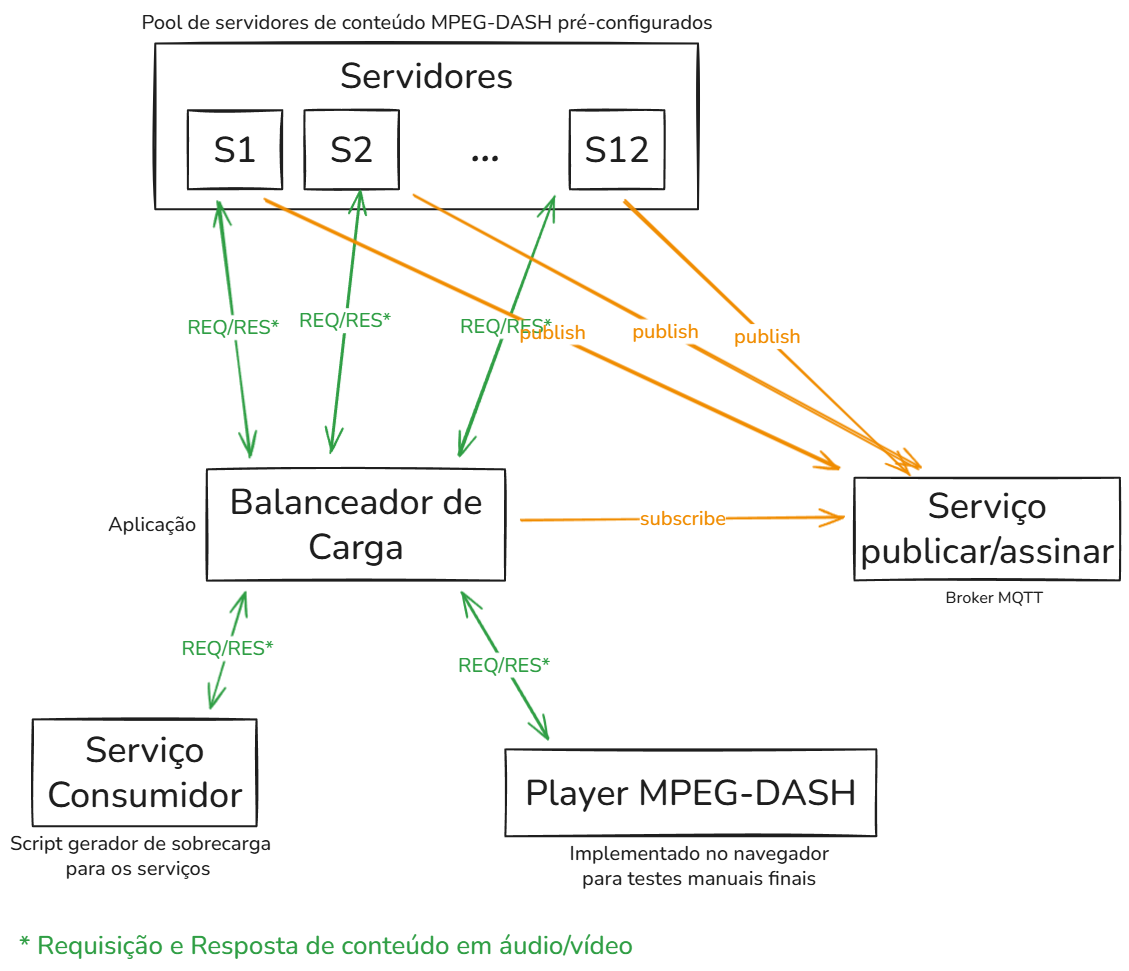
\includegraphics[width=1\linewidth]{TCCI/Textuais/3-Proposta/arch.png}
    \text{Fonte: Elaborado pelo autor (2025)}
    \label{fig:arch}
\end{figure}

% Realização da análise comparativa, dentro do mesmo ambiente simulado, com outros algoritmos de balanceamento de carga
\section{Análise comparativa}

A validação da eficácia do algoritmo proposto será realizada por meio de uma análise comparativa rigorosa, executada em cenários de alta carga. Para estabelecer uma condição de teste relevante, o sistema será submetido a uma carga de trabalho crescente, gerada pelo script cliente que realiza múltiplas requisições paralelas. Este processo será monitorado empiricamente através do player de vídeo final, e o ponto de sobrecarga será definido como o momento em que a degradação da experiência do usuário (QoE), manifestada por travamentos visíveis, torna-se notável. Este mesmo nível de sobrecarga será então utilizado como linha de base para todos os testes comparativos, garantindo a consistência das avaliações.

A metodologia de avaliação será centrada em métricas quantitativas que impactam diretamente a QoE do usuário final. Durante a execução de cada cenário de teste, serão coletados dados sobre: o número total de travamentos (\textit{stalls}) do vídeo, a duração média de cada travamento e o tempo total de ociosidade do serviço (soma de todas as pausas). Essas métricas oferecem uma visão objetiva do desempenho de cada estratégia de balanceamento sob estresse.

O algoritmo proposto, baseado na interpretação de dados obsoletos, será comparado com duas abordagens clássicas e amplamente utilizadas: \textit{Round-Robin} e Seleção Aleatória. Para assegurar uma comparação justa, a mesma aplicação de balanceamento de carga desenvolvida em Rust será utilizada em todos os testes, alterando-se apenas o módulo de decisão do algoritmo. Serão executados os seguintes cenários:

\begin{enumerate}
    \item{Balanceamento com algoritmo Round-Robin.}
    \item{Balanceamento com algoritmo de Seleção Aleatória.}
    \item{Balanceamento com o algoritmo proposto, utilizando um intervalo de atualização dos dados dos servidores de 6 segundos.}
    \item{Balanceamento com o algoritmo proposto, utilizando um intervalo de atualização dos dados dos servidores de 60 segundos.}
    \item{Balanceamento com o algoritmo proposto, utilizando um intervalo de atualização dos dados dos servidores de 600 segundos.}
\end{enumerate}

A hipótese central é que o algoritmo proposto, mesmo com informações consideravelmente desatualizadas (nos intervalos de 60s e 600s), apresentará um desempenho superior em termos de QoE quando comparado aos métodos Round-Robin e Aleatório. Adicionalmente, espera-se que, entre as variações do algoritmo proposto, o intervalo de 6 segundos forneça os melhores resultados, enquanto os intervalos maiores demonstrarão a capacidade do algoritmo de mitigar os efeitos negativos da obsolescência de dados de carga dos servidores envolvidos.

%\ul{acho que deves incluir mais um capítulo com as considerações parciais, onde além de resumir os objetivos e a arquitetura e elencar as próximas atividades, tens uma seção com um cronograma para as atividades a serem desenvolvidas no TCC II}
